Luego de describir el sistema de detección en el Capitulo \ref{cap:sdet}, es posible entender el funcionamiento de los detectores y definir los requisitos para el diseño de la etapa siguiente: el sistema de adquisición de datos, etapa que se encargará de recibir los pulsos digitales provenientes de la interfaz de lectura ASD y del sistema de disparo, con el fin de muestrear los eventos detectados y facilitar la determinación de los vértices de interacción en una posterior etapa de análisis.

En este capítulo se presenta la arquitectura propuesta para la implementación del sistema de adquisición y se detalla el desarrollo de cada una de sus etapas.

\section{Arquitectura propuesta}
\label{sec:arq}

	En el Capítulo \ref{cap:art} se compararon tres sistemas diferentes para la implementación de sistemas de adquisición de datos en el contexto de física de partículas. En diferentes sistemas destacan aspectos comunes de implementación: etapas de detección de eventos, memorias para almacenamiento temporal, procesamiento de los datos y la utilización de FPGAs como la principal herramienta para la implementación del hardware \gcnote{y las otras cosas, memorias y componentes no son hardware?}. Las principales etapas identificadas en los sistemas de adquisición estudiados son: el acondicionamiento de señal, la adquisición misma de los datos, la discriminación de eventos y la comunicación de los datos obtenidos para posteriores análisis.
	
	En sTGC Minería, la etapa de acondicionamiento de señal es realizada mediante la interfaz de lectura ASD ya existente descrita en la Sección \ref{sec:asd} \sgcnote{especificar/recordar si estas ya estaban disenadas o se hizo algo con esto en la memoria}. Las etapas de adquisición, discriminación y comunicación serán entonces las etapas a implementar en el sistema de adquisición de datos desarrollado en este proyecto de titulación.
	
	Los pulsos digitales a adquirir, provenientes de la interfaz ASD, son señales diferenciales LVDS en el orden de los nanosegundos\cite{1999ATLASICs}. Este ancho de pulso tiene correlación con la amplitud del pulso análogo originado en el sistema de detección y el error en su medición implicará menor precisión en la estimación de esta variable, requiriendo un sistema capaz de tener una resolución lo más cercana a 1ns y que permita capturar pulsos de más de 60ns. \sgcnote{poner esto antes de las especificaciones. Las specs deben ser consecuencia de los requerimientos.}
	
	Respecto a la tasa de aparición de pulsos consecutivos, es poco probable que ocurran eventos simultáneos o cercanos. Se espera que el flujo de muones por centímetro cuadrado sea de un muon por minuto\cite{Rocca2018CosmicUs}, lo que en los 15cm$^2$ de área de un strip implicaría cerca de 15 muones por minuto o 0,25E$^{-9}$ muones cada 1ns, traduciéndose en una muy baja probabilidad de eventos simultáneos o cercanos en el tiempo (adyacentes) si se considera por ejemplo una altisima tasa de muestreo de 1GHz. Dado que la tasa de detección de muones disminuye bajo tierra y dado que la toma de una muongrafía conlleva un tiempo prolongado de exposición a rayos cósmicos, se concluye que ignorar posibles eventos simultáneos o adyacentes no tendrá implicancias significativas en los resultados de la muongrafía final. \sgcnote{lo mismo anterior.}
	
	Tomando como antecedente los objetivos del proyecto descritos en la Sección \ref{sec:planteamiento}, junto con las características del sistema de detección descrito en el Capítulo \ref{cap:sdet} y las especificaciones descritas en los parrafos anteriores, se definen lo siguientes requisitos para el diseño del sistema de adquisición de datos para detectores de muones:
	
	\begin{itemize}
		\item Debe incluir al menos 16 entradas compatibles con el estándar LVDS, con el fin de conectar al menos una interfaz de lectura ASD asociada a un detector de 16 canales.
		\item Es importante contar con un reloj presente o sintetizable de una frecuencia mayor a 100MHz, siendo lo más cercano a 1GHz posible \sgcnote{por que estos numeros}, con el fin de captar la duración de los pulsos y el momento de aparición de un evento con la mayor precisión disponible.
		\item Se debe considerar que la señal de disparo que entrará al sistema estará desfasada cerca de 125ns\cite{Oyanadel2020SistemaSTGC} respecto al paso real de los muones a través el detector, siendo necesaria la implementación un sistema capaz de asociar la simultaneidad de eventos detectados con la señal de disparo.
		\item  Se debe tener la capacidad de mantener sincronizadas las señales de detección y disparo, además de guardar la información en memorias temporales.
		\item Es requisito que la implementación del sistema de adquisición permita escalamiento para agregar nuevos detectores adyacentes con el fin de aumentar el área de prueba o para leer detectores superpuestos.
	\end{itemize}
	
	

	\subsection{Esquema General del Sistema de Adquisición Propuesto}
		Como se indica en la figura \ref{img:diagrama}, se requieren al menos tres etapas esenciales: adquirir, discriminar y comunicar. Adquirir corresponde a muestrear las señales digitales asociadas a eventos de detección y mantenerlas en memoria hasta ser discriminadas. Discriminar se refiere a descartar aquellos eventos que no corresponden a la interacción de un muon con el detector leyendo la señal de disparo. Comunicar corresponde a enviar los datos de eventos seleccionados hacia un dispositivo externo, para así almacenarlos o analizarlos. En las secciones siguientes se describe el dónde y cómo implementar cada una de estas tres etapas.
		
		\begin{figure}[h]
			\centering
			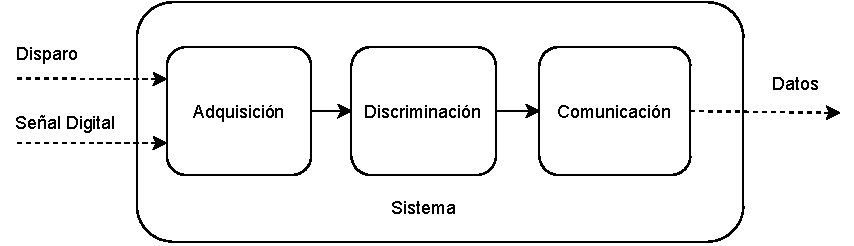
\includegraphics[scale=0.9]{basico.pdf}
			\caption{Diagrama del esquema general para el sistema de adquisición a diseñar. El disparo corresponde a la señal digital que indica si la partícula detectada es un muon, mientras que la señal digital corresponde al pulso captado por el detector, luego de haber pasado por la interfaz de lectura. Los datos son la información asociada a eventos seleccionados, que serán enviados a un dispositivo externo.}
			\label{img:diagrama}
		\end{figure}
	
	\subsection{Plataforma}
		Según los casos de estudio presentados en el Capítulo \ref{cap:art}, la alternativa más utilizada para la implementación de hardware \gcnote{especificar propiedades del hardware a implementa en la FPGA.} es la FPGA, herramienta que se ha visto con mayor frecuencia en proyectos relativos a física de partículas y adquisición de datos. Las FPGAs cuentan con una cantidad significativa de recursos y periféricos, incluyendo además hardware dedicado para comunicación, serialización y almacenamiento de datos. Una desventaja conocida corresponde a que se basan en memorias volátiles, por lo que el hardware descrito debe ser reconfigurado cada vez que se enciende, por lo que los datos importantes deben ser almacenados en memorias externas.
		
		Dado que el laboratorio de electrónica en CCTVal cuenta con placas de desarrollo marca Trenz \gcnote{Da un poco mas de contexto sobre el uso de Trenz. No es solo porque \emph{es lo que hay}.}, en este proyecto de titulación se utilizará un módulo Trenz TE0720 \cite{TrenzElectronic2020TE0720Wiki} montado en una tarjeta de desarrollo Trenz TE0703 \cite{TrenzElectronic2019TE0703Wiki}, ambas ilustradas en la Figura \ref{fig:trenz}. El módulo TE0720 contiene un SoC (System on a Chip) Xilinx Zynq 7000 \cite{Xilinx2012Zynq-7000Architecture} que incluye lógica programable (PL) equivalente a una FPGA Xilinx Artix 7\cite{Xilinx20107DS180} y un procesador (PS) ARM Cortex Cortex-A9 de dos núcleos, con múltiples periféricos como memoria flash, comunicación UART y un GPIO (General Purpose Input/Output) de 32 bits.
		
		Una de las principales ventajas de usar el módulo TE0720 es que permite concentrar todo el diseño de hardware en un solo lugar sin necesidad de FPGAs o ASICs adicionales, ya que posee 85.000 celdas lógicas, 4.9Mb de Block RAM, una frecuencia de reloj de 33.3MHz con hasta 600MHz sintetizables y 152 puertos de entrada y salida compatibles con el estándar LVDS, suficientes como para conectar hasta 4 interfaces de lectura ASD. Este módulo también destaca por ser una plataforma flexible, en el sentido de brindar las posibilidades de adaptar el diseño propuesto sin tener que adquirir nuevo equipamiento. Esta versatilidad es intrínseca de las FPGAs, las cuales se caracterizan por permitir un gran control en el diseño del hardware a bajo nivel. Finalmente, al ser una tecnología conocida en CCTVal, se cuenta con acceso a su documentación, lo que facilita el desarrollo del hardware en esta plataforma por sobre otras alternativas comerciales.
		
		\begin{figure}[H]
			\centering
			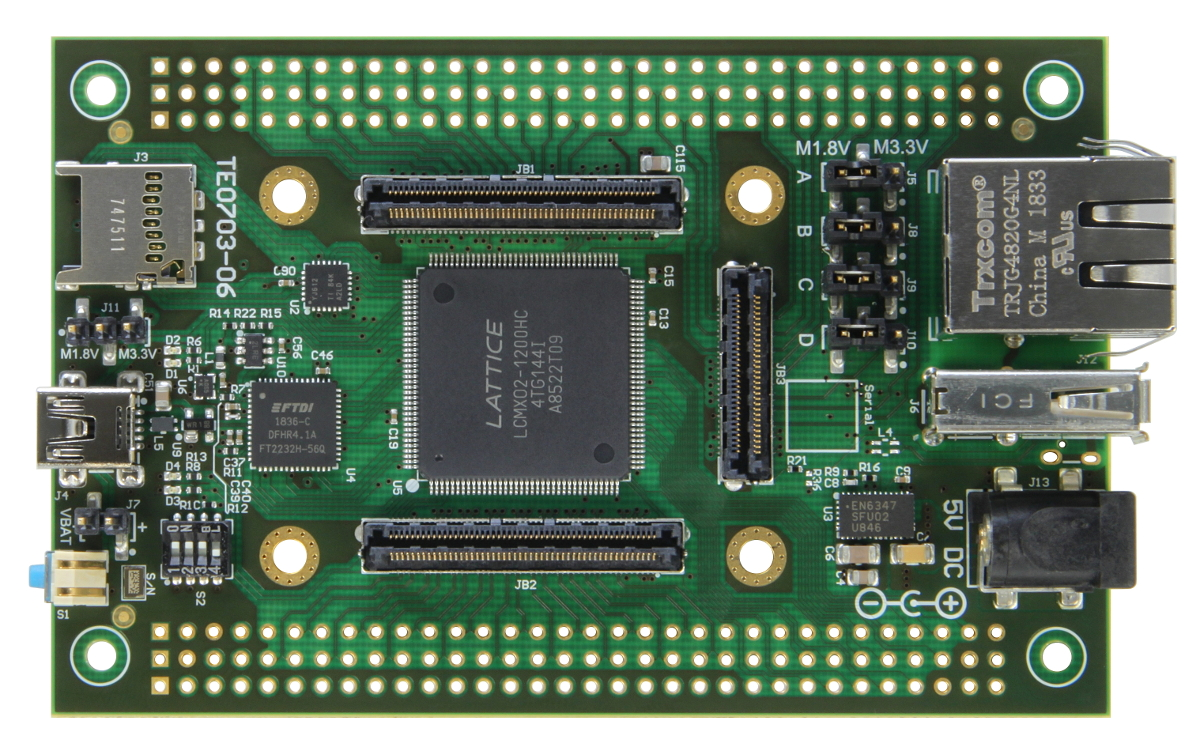
\includegraphics[scale=0.23]{TE0703-06_1.jpg}
			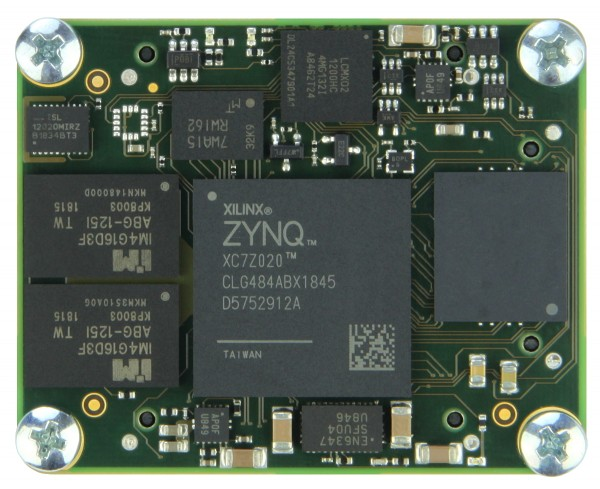
\includegraphics[scale=0.25]{TE0720-03-62I12GA-_1}
			\caption{Tarjeta de desarrollo y módulo Zynq a utilizar. A la izquierda se ilustra la placa de desarrollo Trenz TR0703\cite{TrenzElectronic2019TE0703Wiki} y a su derecha se ilustra el módulo que va montado en ella: Trenz TR0720\cite{TrenzElectronic2020TE0720Wiki} que contiene un SoC Zynq 7000\cite{}.}
			\label{fig:trenz}
		\end{figure}
	
	\subsection{Propuesta}
		La arquitectura del sistema de adquisición que se implementará en el módulo Trenz se ilustra en la Figura \ref{fig:muon-daq}. Se propone utilizar un módulo de muestreo (\textit{sampler}), un buffer de eventos (\textit{Event Buffer}, FIFO), un módulo de lectura para comunicar los datos (\textit{Event Reader}), y un módulo de comunicación implementado en el procesador (GPIO, UART). Este sistema permite la adquisición de datos provenientes de un solo detector de muones, conectándose directamente a la interfaz ASD y a la señal generada por el sistema de disparo.
		
		El módulo \textit{Sampler} se encarga de muestrear los 16 pulsos LVDS provenientes de la interfaz ASD a la máxima frecuencia de reloj posible, para mantenerlos en un registro de desplazamiento (shift register) utilizado como buffer de datos. En este registro se mantendrán los datos muestreados a la espera de la señal de disparo para ser traspasados al siguiente módulo. Mientras no llegue la señal de disparo, los datos seguirán avanzando en el registro de desplazamiento, descartando automáticamente los datos más antiguos.
		
		El \textit{Event Buffer} se encarga de tomar los datos coincidentes con la señal de disparo y los almacena en una memoria FIFO (First In, First Out)\cite{XilinxFIFOSuite}. En esta memoria FIFO se guardan los eventos por orden de llegada, almacenando los datos asociados a cada canal de manera consecutiva. Es decir, cada vez que un evento es almacenado, se utilizan 16 direcciones de memoria, una para cada canal del evento guardado.
		
		El módulo \textit{Event Reader} lee los datos almacenados en la memoria FIFO y los envía hacia el módulo de comunicación mediante el GPIO del procesador. La lectura de los datos inicia al recibir la solicitud desde el módulo de comunicación a través del GPIO. Una vez leídos los datos, estos son enviados a un computador externo (PC) para su almacenamiento definitivo y posterior análisis.
		
		Para un futuro escalamiento del sistema, con el fin de conectar más detectores de muones, bastaría con replicar los módulos \textit{Sampler}, \textit{Event Buffer} y FIFO, ajustando a la vez el módulo \textit{Event Reader} y el módulo de comunicación, para así coordinar la lectura de cada una de las memorias FIFO asociadas a cada detector.
		
		
		\begin{figure}[H]
			\centering
			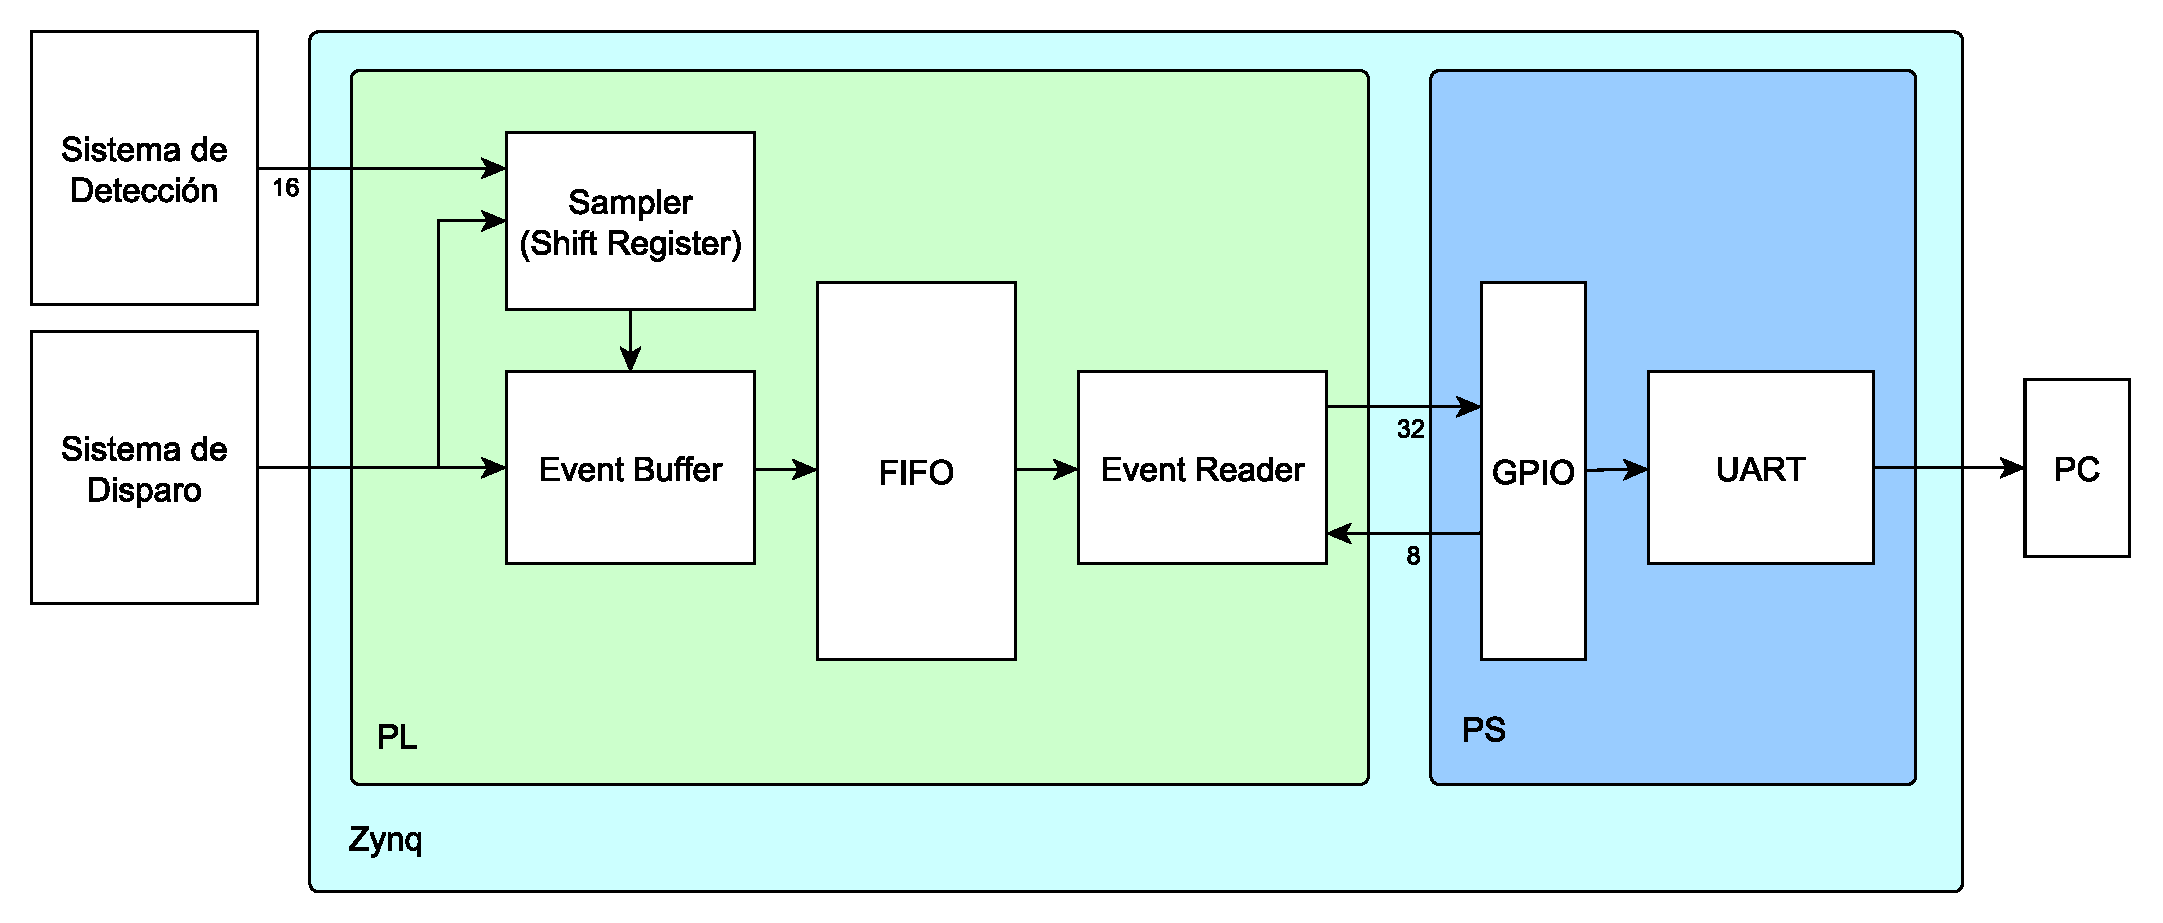
\includegraphics[scale=0.38]{muon-daq.pdf}
			\caption{Diagrama de la arquitectura de hardware propuesta para el diseño de un sistema de adquisición de datos asociado a un solo detector de muones.}
			\label{fig:muon-daq}
		\end{figure}
		
\section{Implementación del Sistema de Adquisición}
	La implementación del sistema de adquisición de datos en el módulo TE0720 se realizó mediante el software Vivado Design Suite 2019.1 y Vivado SDK 2019.1 \sgcnote{version} para la descripción de hardware en lógica programable y  para la programación de software en el procesador, respectivamente. En esta sección se presenta el funcionamiento general de cada módulo y el detalle técnico de implementación se encuentra disponible en el repositorio Github en \url{https://github.com/jairoegc/muon-daq}.
	
	La descripción de hardware se llevó a cabo en el HDL (Hardware Description Language) SystemVerilog y la integración de cada módulo se hizo mediante \textit{Block Design}, correspondiente a un método de descripción de hardware en formato de diagrama de bloques, el cual permite automatizar algunos procesos de instanciación de módulos e interconexión de puertos. En la Figura \ref{fig:blockdesign} \gcnote{no se ve bien por temas de escala. Podrias dejarla en una sola pagina en formato lateral.} se ilustra el diagrama de bloques del sistema de adquisición implementado en el módulo TE0720, donde se observan los diferentes bloques utilizados. El bloque \textit{ZYNQ7 Processing System} corresponde al procesador, donde se ubica el módulo de comunicación. El bloque \textit{top\_wrapper} agrupa los módulos \textit{Sampler, Event Reader y Event Buffer}, que junto con los bloques \textit{FIFO Generator}, \textit{Clocking Wizard} y \textit{clk\_divider} corresponden a los módulos implementados en la lógica programable. Los módulos \textit{AXI GPIO} corresponden a los puertos de entrada de datos y salida de comandos del sistema de comunicación incluido al interior del procesador, donde el módulo \textit{axi\_gpio\_0} está asociado a los 32bits de entrada de datos, mientras que el módulo \textit{axi\_gpio\_1} corresponde a los 8 bits de salida para comandos de lectura. Los bloques \textit{Processor System Reset} y \textit{AXI Interconnect} son módulos auxiliares instanciados de manera automática por el software y permiten generar las señales de reset y habilitar la comunicación con la GPIO del procesador respectivamente. Por último, la señal \textit{trigger} corresponde a la señal de disparo, mientras que los arreglos de señales \textit{Ch\_A\_P[15:0]} y \textit{Ch\_A\_N[15:0]} corresponden a los puertos de entrada para las señales de detección LVDS con sus terminales positivos y negativos respectivamente.
	
	\begin{figure}[H]
		\centering
		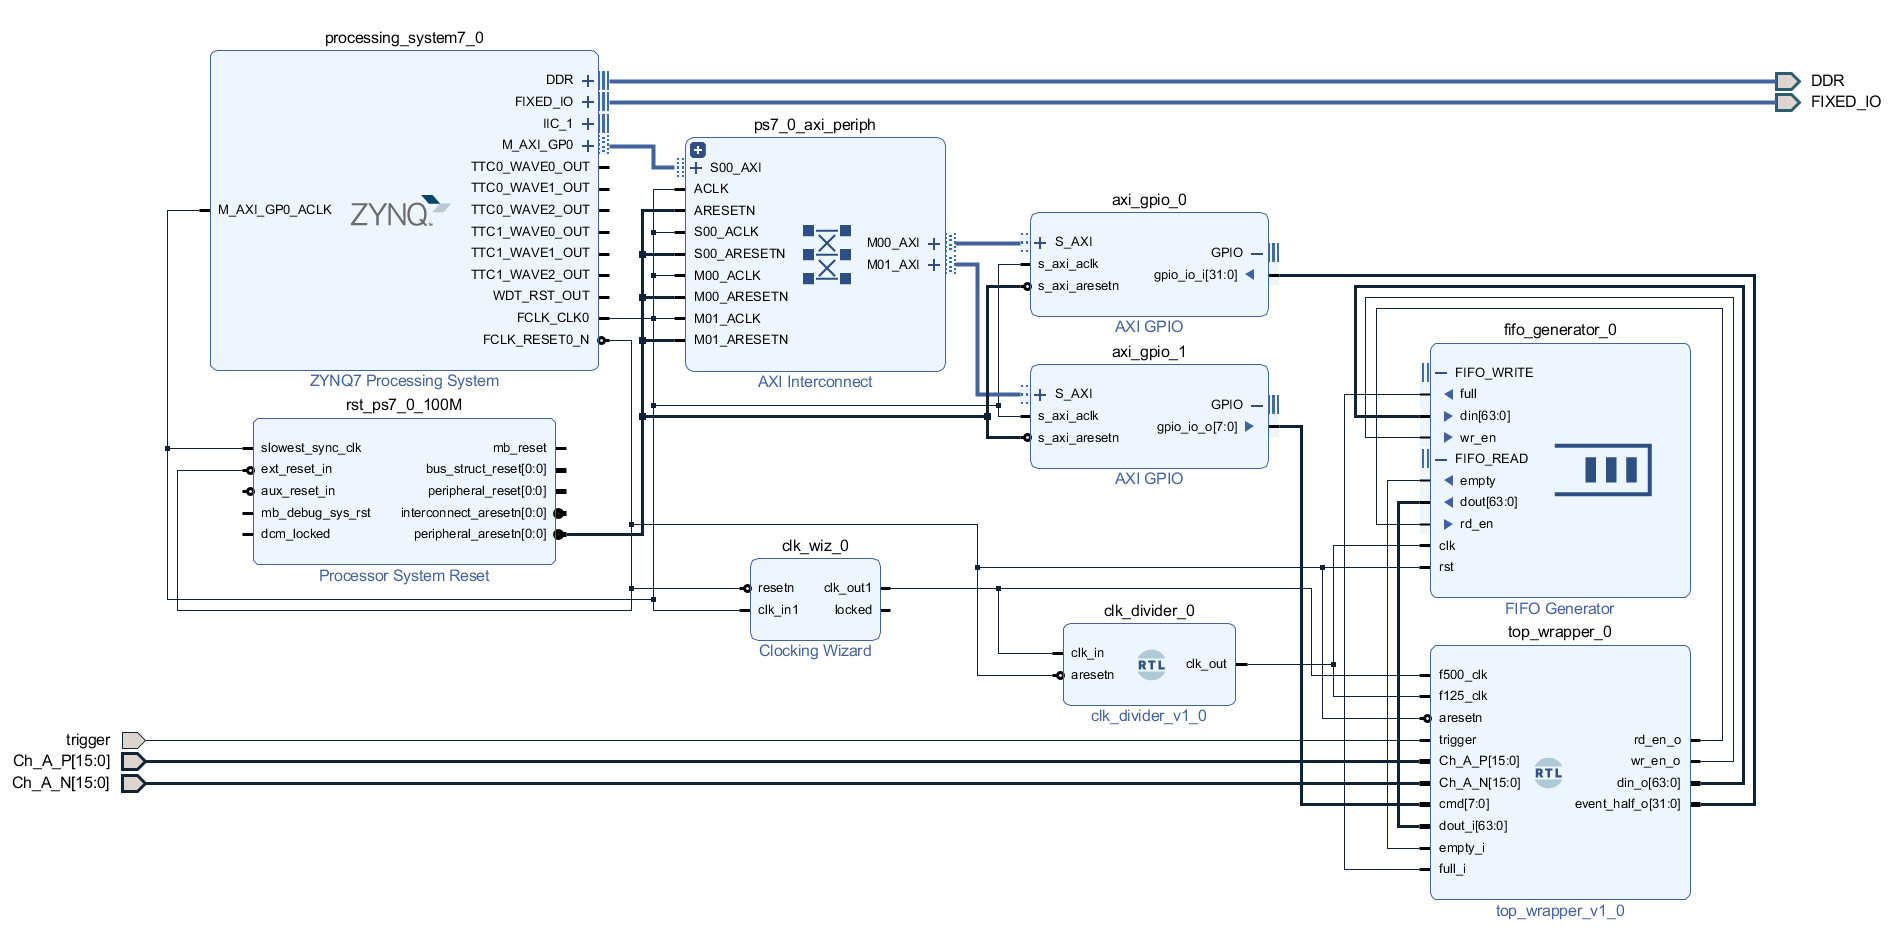
\includegraphics[scale=0.28]{blockdesign.png}
		\caption{Block Design del sistema de adquisición de datos implementado en el módulo TE0720.}
		\label{fig:blockdesign}
	\end{figure}
	
	A continuación se detalla del desarrollo de cada módulo, su funcionamiento, los puertos asociados y sus diagramas pertinentes. \gcnote{discutir detalles tecnicos una vez este entregado el informe.}
	
	\subsection{Sampler}
	\label{sec:sampling}
	
	El módulo \textit{Sampler} corresponde a la etapa de muestreo y discriminación, encargándose de recibir las señales digitales generadas por la interfaz ASD. Esta etapa muestrea cada señal entrante y asocia los datos a la señal de disparo correspondiente. Los principales objetivos de este módulo son:
	
	\begin{itemize}
		\item Muestrear\sgcnote{cuanto es maxima frecuencia?} los pulsos digitales la frecuencia lo más cercana a 600MHz (máxima frecuencia sintetizable en la plataforma de desarrollo).
		\item Mantener en memoria los pulsos muestreados mientras llega la señal de disparo.
		\item Transferir los pulsos muestreados hacia la etapa siguiente al momento de detectar la señal de disparo.
	\end{itemize}

	Para interconectar la interfaz ASD con la tarjeta de desarrollo, se identificaron los conectores de cada dispositivo y se les asignaron etiquetas. Para el caso de la interfaz ASD se le asignó la letra ``A'' por ser la primera en ser conectada, nombrándose cada señal como ``JA-n'', donde ``n'' corresponde al número del pin de cada señal ubicada en el conector de 40 posiciones según la Figura \ref{img:asd-ports} de la Sección \ref{sec:asd}.
	
	En el caso de la tarjeta de desarrollo Trenz TE0703\sgcnote{especifica que te refieres a la trenz}, esta cuenta con dos conectores tipo VG96. La nomenclatura para cada pin se ilustra en la Figura \ref{fig:trenz-layout}, destacándose en rojo los pines escogidos para interconectar la interfaz ASD. Estos pines se escogieron estratégicamente con el fin de estar ubicados en un extremo accesible, con puertos cercanos entre si, ordenados de manera consecutiva, y dejando espacio disponible para conectar otros detectores en el futuro.
	
	\begin{figure}[H]
		\centering
		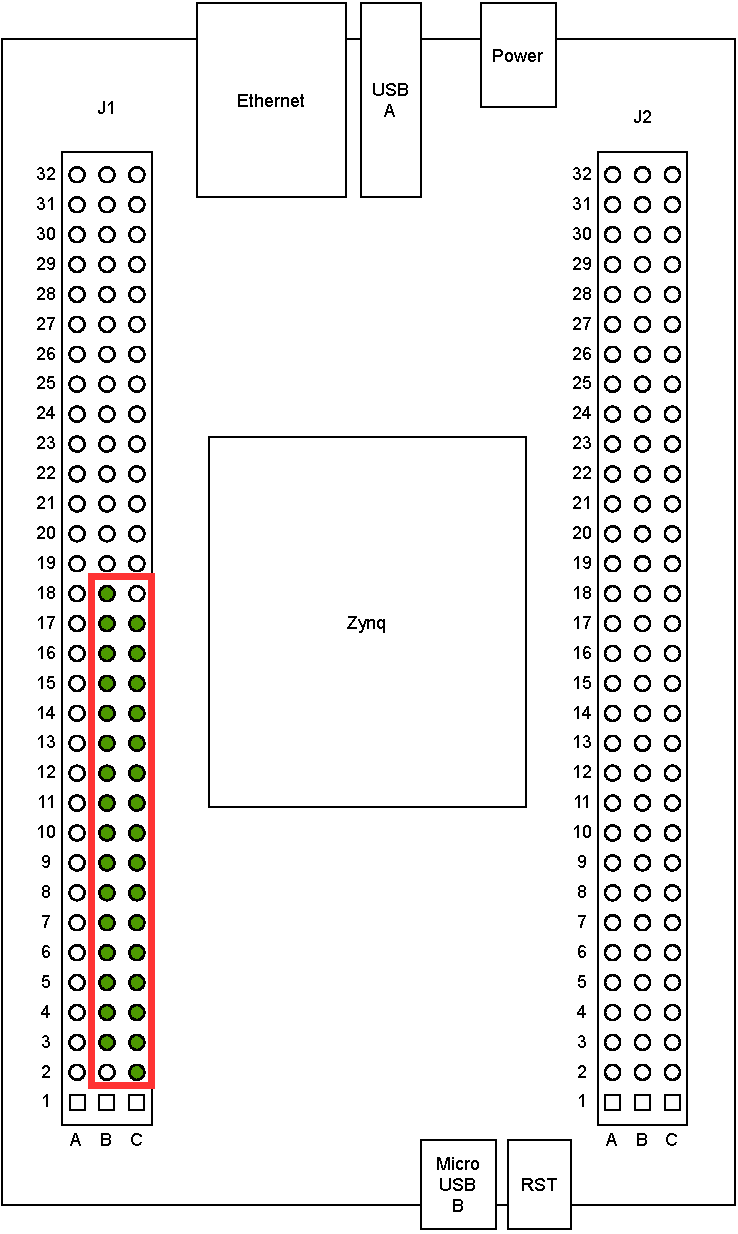
\includegraphics[scale=0.7]{trenz-layout}
		\caption{Diagrama de la vista superior de la tarjeta de desarrollo utilizada, indicando la nomenclatura de los pines correspondientes a sus conectores VG96. Los pines utilizados para conectar la interfaz ASD se encuentran enmarcados en el recuadro rojo. \hl{el cuadro rojo se sobrepone a los circulos, no queda clara el area de interes.}}
		\label{fig:trenz-layout}
	\end{figure}
	
	En la lógica programable, cada señal se recibe en los arreglo de puertos ``Ch\_A\_P[15:0]'' y ``Ch\_A\_N[15:0]'', donde ``Ch'' significa canal, ``A'' indica que corresponden la interfaz de lectura ``A'', ``P'' indica que son señales de polaridad positiva y ``N'' significa que son señales de polaridad negativa.
	
	En base a las nomenclaturas anteriores e incluyendo los propios nombres de los pines descritos en los esquemáticos eléctricos de la tarjeta de desarrollo TE0703\cite{TrenzElectronicGmbHTE0703SCH-TE0703-06} y los pines internos de la Zynq, se realizó la interconexión ASD-Zynq según lo indicado en la Tabla \ref{tab:zynq-asd}.
	
	\begin{table}[]
		\centering
		\resizebox{\textwidth}{!}{%
			\begin{tabular}{|c|c|c|c|c|c|}
				\hline
				\rowcolor[HTML]{4472C4} 
				\multicolumn{1}{|l|}{\cellcolor[HTML]{4472C4}{\color[HTML]{FFFFFF} \textbf{Zynq Pin}}} &
				\multicolumn{1}{l|}{\cellcolor[HTML]{4472C4}{\color[HTML]{FFFFFF} \textbf{Sch. Name}}} &
				\multicolumn{1}{l|}{\cellcolor[HTML]{4472C4}{\color[HTML]{FFFFFF} \textbf{Conn. VG96}}} &
				\multicolumn{1}{l|}{\cellcolor[HTML]{4472C4}{\color[HTML]{FFFFFF} \textbf{Conn. 40p ASD}}} &
				\multicolumn{1}{l|}{\cellcolor[HTML]{4472C4}{\color[HTML]{FFFFFF} \textbf{Channel}}} &
				\multicolumn{1}{l|}{\cellcolor[HTML]{4472C4}{\color[HTML]{FFFFFF} \textbf{Array}}} \\ \hline
				\rowcolor[HTML]{D9E1F2} 
				F16 & B35\_L1\_P  & J1-C2  & JA-9  & 0  & Ch\_A\_P{[}0{]}  \\ \hline
				E16 & B35\_L1\_N  & J1-C3  & JA-10 & 0  & Ch\_A\_N{[}0{]}  \\ \hline
				\rowcolor[HTML]{D9E1F2} 
				G17 & B35\_L6\_P  & J1-B3  & JA-11 & 1  & Ch\_A\_P{[}1{]}  \\ \hline
				F17 & B35\_L6\_N  & J1-B4  & JA-12 & 1  & Ch\_A\_N{[}1{]}  \\ \hline
				\rowcolor[HTML]{D9E1F2} 
				E15 & B35\_L3\_P  & J1-C4  & JA-13 & 2  & Ch\_A\_P{[}2{]}  \\ \hline
				D15 & B35\_L3\_N  & J1-C5  & JA-14 & 2  & Ch\_A\_N{[}2{]}  \\ \hline
				\rowcolor[HTML]{D9E1F2} 
				F18 & B35\_L5\_P  & J1-B5  & JA-15 & 3  & Ch\_A\_P{[}3{]}  \\ \hline
				E18 & B35\_L5\_N  & J1-B6  & JA-16 & 3  & Ch\_A\_N{[}3{]}  \\ \hline
				\rowcolor[HTML]{D9E1F2} 
				G19 & B35\_L20\_P & J1-C6  & JA-17 & 4  & Ch\_A\_P{[}4{]}  \\ \hline
				F19 & B35\_L20\_N & J1-C7  & JA-18 & 4  & Ch\_A\_N{[}4{]}  \\ \hline
				\rowcolor[HTML]{D9E1F2} 
				F21 & B35\_L23\_P & J1-B7  & JA-19 & 5  & Ch\_A\_P{[}5{]}  \\ \hline
				F22 & B35\_L23\_N & J1-B8  & JA-20 & 5  & Ch\_A\_N{[}5{]}  \\ \hline
				\rowcolor[HTML]{D9E1F2} 
				G15 & B35\_L4\_P  & J1-C8  & JA-21 & 6  & Ch\_A\_P{[}6{]}  \\ \hline
				G16 & B35\_L4\_N  & J1-C9  & JA-22 & 6  & Ch\_A\_N{[}6{]}  \\ \hline
				\rowcolor[HTML]{D9E1F2} 
				C17 & B35\_L11\_P & J1-B9  & JA-23 & 7  & Ch\_A\_P{[}7{]}  \\ \hline
				C18 & B35\_L11\_N & J1-B10 & JA-24 & 7  & Ch\_A\_N{[}7{]}  \\ \hline
				\rowcolor[HTML]{D9E1F2} 
				E19 & B35\_L21\_P & J1-C10 & JA-26 & 8  & Ch\_A\_P{[}8{]}  \\ \hline
				E20 & B35\_L21\_N & J1-C11 & JA-25 & 8  & Ch\_A\_N{[}8{]}  \\ \hline
				\rowcolor[HTML]{D9E1F2} 
				B16 & B35\_L8\_P  & J1-B11 & JA-27 & 9  & Ch\_A\_P{[}9{]}  \\ \hline
				B17 & B35\_L8\_N  & J1-B12 & JA-28 & 9  & Ch\_A\_N{[}9{]}  \\ \hline
				\rowcolor[HTML]{D9E1F2} 
				D16 & B35\_L2\_P  & J1-C12 & JA-29 & 10 & Ch\_A\_P{[}10{]} \\ \hline
				D17 & B35\_L2\_N  & J1-C13 & JA-30 & 10 & Ch\_A\_N{[}10{]} \\ \hline
				\rowcolor[HTML]{D9E1F2} 
				G20 & B35\_L22\_P & J1-B13 & JA-31 & 11 & Ch\_A\_P{[}11{]} \\ \hline
				G21 & B35\_L22\_N & J1-B14 & JA-32 & 11 & Ch\_A\_N{[}11{]} \\ \hline
				\rowcolor[HTML]{D9E1F2} 
				A21 & B35\_L15\_P & J1-C14 & JA-33 & 12 & Ch\_A\_P{[}12{]} \\ \hline
				A22 & B35\_L15\_N & J1-C15 & JA-34 & 12 & Ch\_A\_N{[}12{]} \\ \hline
				\rowcolor[HTML]{D9E1F2} 
				B21 & B35\_L18\_P & J1-B15 & JA-35 & 13 & Ch\_A\_P{[}13{]} \\ \hline
				B22 & B35\_L18\_N & J1-B16 & JA-36 & 13 & Ch\_A\_N{[}13{]} \\ \hline
				\rowcolor[HTML]{D9E1F2} 
				H22 & B35\_L24\_P & J1-C16 & JA-37 & 14 & Ch\_A\_P{[}14{]} \\ \hline
				G22 & B35\_L24\_N & J1-C17 & JA-38 & 14 & Ch\_A\_N{[}14{]} \\ \hline
				\rowcolor[HTML]{D9E1F2} 
				A18 & B35\_L10\_P & J1-B17 & JA-39 & 15 & Ch\_A\_P{[}15{]} \\ \hline
				A19 & B35\_L10\_N & J1-B18 & JA-40 & 15 & Ch\_A\_N{[}15{]} \\ \hline
			\end{tabular}%
		}
		\caption{Mapeo de conexiones entre Zynq e interfaz ASD. }
		\label{tab:zynq-asd}
	\end{table}
	
	Una vez definida la nomenclatura de puertos, es posible interconectar las tarjetas y proceder con la toma de muestras. Para capturar las señales LVDS, se declaran puertos IBUFDS (Input Buffer for Differential Signals) \cite{Xilinx2012XilinxDesigns} en la lógica programable, configurándolos para recibir señales LVDS de 2.5V y activando la resistencia interna de 100$\Omega$ para adaptar la terminación al estándar diferencial. Luego de ser capturar las señales, estas se sincronizan con el reloj del circuito pasando a través de dos Flip-flops consecutivos (Synchonizer).
	
	El muestreo \sgcnote{typo. Revisr cuidadosamente todo el texto. Ya habia corregido directamente un par.} de las señales se realiza a 400MHz por ser la frecuencia más alta sintetizable antes de producir errores de \textit{timing} \gcnote{especificar un poco mas sobre timing.}, además de dar una resolución de tiempo de 2,5ns para distinguir el ancho de los pulsos digitales. Esta resolución cumple con los requisitos descritos en la Sección \ref{sec:arq}.
	
	El método de muestreo utilizado consiste en un shift-register de 64 bits, el cual representa la ventana de adquisición del pulso digital capturado. Los 64 bits de este shift-register serán entregados a la siguiente etapa en el instante en que se reciba la señal de disparo. Considerando 16 canales con un buffer de 64 bits cada uno, el shift-register consiste en un arreglo bidimensional de 16 filas con 64 bits de ancho cada una.
	
	El shift-register funciona como buffer y retardo para la señal digital muestreada. Dada la frecuencia de muestreo, cada bit representa 2,5ns de la señal muestreada. Considerando que la señal de disparo posee un retardo de 100ns, a la llegada del disparo la señal queda ubicada entre el bit 24 y 63 aproximadamente. Esta configuración permite una ventana de 30ns antes de la señal de disparo y permite el muestreo de señales de hasta 130ns de duración. Se utiliza un shift-register debido a su simplicidad, su capacidad de operar a altas frecuencias de reloj y por permitir el almacenamiento natural por orden de llegada de cada bit digital de la la señal, haciendo posible entregar la totalidad de los datos contenidos en este shif-register a la etapa siguiente.
	
	Al detectar la señal de disparo, esta etapa registra los datos de todos los canales en un arreglo bidimencional y mantiene su estado hasta recibir la señal de que han sido guardados correctamente por la etapa siguiente. Mientras esto no suceda, el shift-register seguirá muestreando datos, pero se ignorarán las señales de disparo.
	
	La Figura \ref{fig:sampler} ilustra un diagrama simplificado del módulo \textit{sampler} considerando la lógica para una sola señal LVDS entrante. \sgcnote{especificar en alguna parte, quizas al inicio de la seccion o capitulo, que la descripcion entregada en el informe escrito es simplificada para dar un contexto, pero la implementacion se encuentra en un repositorio donde se pueden ver todos los detalles tecnicos.}
	
	\begin{figure}[H]
		\centering
		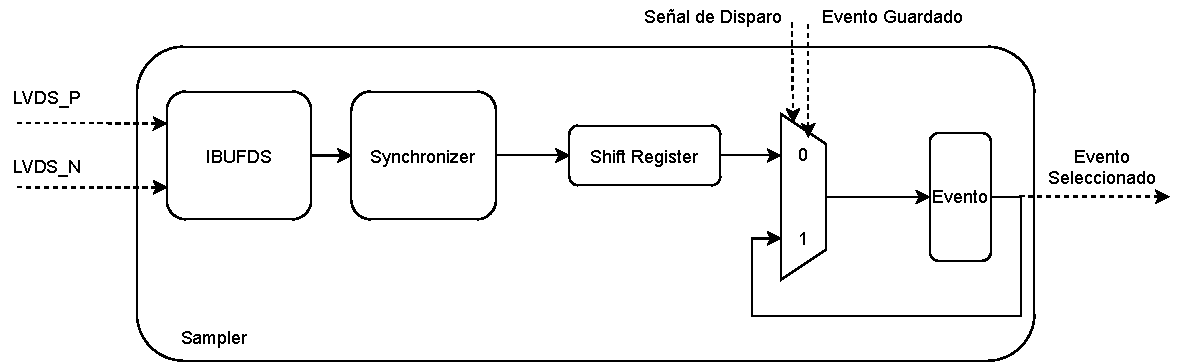
\includegraphics[scale=0.7]{sampler.pdf}
		\caption{Diagrama simplificado del módulo \textit{Sampler}, ejemplificado para una sola señal LVDS.}
		\label{fig:sampler}
	\end{figure}
	
	
	\subsection{Event Buffer}
	\label{sec:buffer}
	
	El buffer de eventos se encarga de almacenar provisoriamente los eventos entrantes en una memoria FIFO hasta que la etapa siguiente solicite la entrega de los eventos capturados. El buffer funciona a 100MHz, dado que la memoria FIFO no es capaz de trabajar a altas frecuencias de reloj.
	
	Si se recibe una señal de disparo, el \textit{Event Buffer} procede a leer los datos provenientes de la etapa anterior (\textit{sampler}). En cada ciclo de reloj se guarda en la memoria FIFO la última fila del arreglo bidimensional que representa al evento seleccionado. Una vez que la información es almacenada en memoria, se desplazan los datos del arreglo bidimensional (Shift) y se repite el ciclo 16 veces. Así, en la memoria FIFO cada dirección de memoria corresponderá a canales consecutivos de un mismo evento, donde cada canal es representado en 64 bits de datos. Se decidió operar de esta manera para simplificar la implementación del hardware y debido a que no es posible almacenar un arreglo bidimensional en una sola dirección de memoria FIFO. Además, se escogió una memoria FIFO para implementar este buffer por adecuarse bien a la naturaleza de los datos: el orden de los eventos es importante y con esta memoria los eventos son leídos por orden de llegada. Además, esta memoria permite el almacenamiento de mas de 50 eventos y sus respectivos canales.
	
	La Figura \ref{fig:event-buffer} ilustra el módulo \textit{Event Buffer} de manera simplificada, ejemplificando el flujo de información desde el evento seleccionado por el módulo \textit{sampler} hasta la fila de 64bits a ser guardada en la memoria FIFO por cada ciclo de reloj hasta completar las 16 filas que componen el evento que está siendo guardado. Existe un contador que lleva la cuenta de las veces que se ha desplazado el arreglo bidimensional que contiene al evento y cuenta con lógica combinacional que coordina el flujo de la información. El módulo emite una señal para indicarle al módulo \textit{Sampler} que el evento ha sido guardado por completo en la memoria FIFO.
	
	\begin{figure}[H]
		\centering
		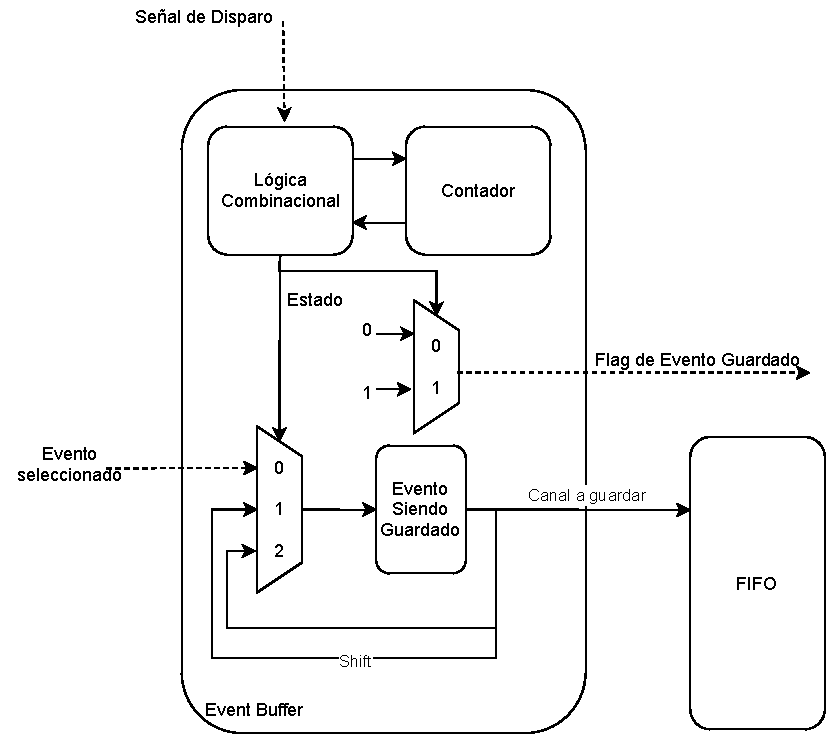
\includegraphics[scale=0.7]{event-buffer.pdf}
		\caption{Diagrama simplificado del módulo \textit{Event Buffer}.}
		\label{fig:event-buffer}
	\end{figure}
	
	\subsection{Event Reader y Comunicación}
	\label{sec:comm}
	El modulo \textit{Event Reader}, ilustrado en el costado izquierdo de la Figura \ref{fig:com} cumple la función de leer los eventos almacenados en la memoria FIFO cada vez que reciba un comando de 8 bits desde el módulo de comunicación. Al recibir el comando, el módulo comienza a leer cada dirección de la memoria FIFO hasta leer las 16 direcciones consecutivas que componen a un mismo evento. Cada dirección almacena un canal de detección en 64bits, pero el \textit{Event Reader} separa esta información en 2 paquetes de 32bits cada uno, demorando dos ciclos de reloj por cada canal que se desee enviar. Este formato de entrega permite la comunicación entre la lógica programable y el procesador mediante el GPIO, utilizando un puerto de precisamente 32bits. Dado que el GPIO del procesador cuenta con puertos limitados, no es posible utilizar un puerto de 64Bits de manera directa, debiendo realizarse en dos pasos. Por otro lado, los datos se entregan desde la PL al PS y no al revés debido a que el módulo de comunicación UART (Universal Asynchronous Receiver-Transmitter) está ubicado en el procesador, mientras que los datos están almacenados en la lógica programable.
	 
	Complementariamente, la etapa de comunicación ilustrada en el costado derecho de la Figura \ref{fig:com} se encarga de entregar los eventos recibidos desde el \textit{event reader} hacia el mundo exterior mediante la UART presente el procesador de la Zynq, a una tasa de transferencia de 115.200bps (baudios por segundo). Este módulo recibe comandos en formato ASCII desde un computador externo (que serán traspasados al módulo \textit{event reader}) y entrega los datos provenientes de la lógica programable al computador solicitante en forma de números enteros sin signo de 32bits.
	
	\begin{figure}[H]
		\centering
		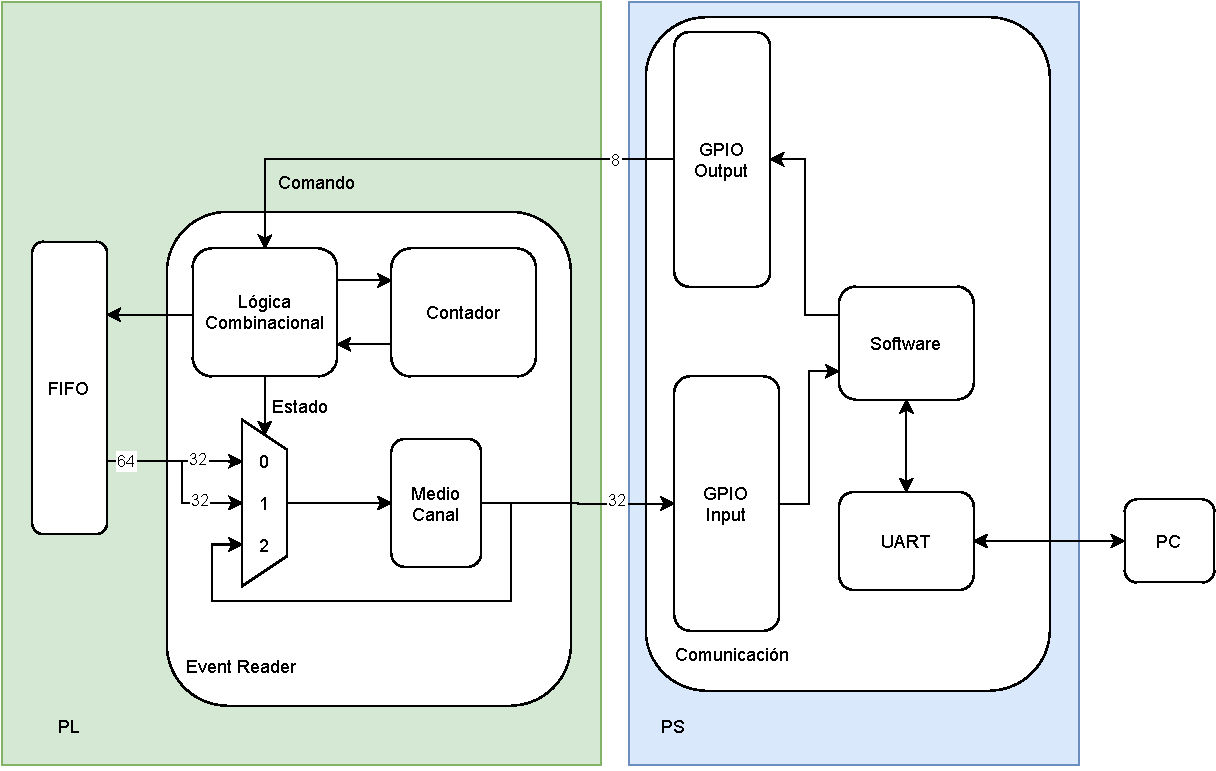
\includegraphics[scale=0.67]{com.pdf}
		\caption{Diagrama simplificado del módulo \textit{Event Reader} y el módulo de comunicación en el procesador.}
		\label{fig:com}
	\end{figure}
	
	Siendo estas todas las etapas del sistema de adquisición de datos, es posible operar el sistema y capturar pulsos de prueba, leer los datos muestreados y contrastar la integridad de la información entre los pulsos iniciales y los datos leídos por comunicación serial.
	
	
	
